\chapter{Plataformas de desarrollo y herramientas utilizadas}
\label{cap:capitulo3}

En el capitulo que a continuación se presenta se van a describir las distintas plataformas y herramientas que se han utilizado a lo largo desarollo de este \ac{TFG}

\section{Lenguajes de programación}
\label{sec:lenguajes_programacion}

\subsection{Python}
\label{subsec:python}

Python es un lenguaje de programación orientado a objetos, de alto nivel y fácil de interpretar, con una sintaxis sencilla y legible \cite{que_es_python_1}. Actualmente, es uno de los lenguajes de programación más populares y resulta especialmente útil para el desarrollo de prototipos. Esto se debe a su facilidad de uso, que permite codificar algoritmos complejos de manera rápida y ágil. Además, es muy utilizado para desarrollar aplicaciones y algoritmos de inteligencia artificial, gracias a la gran cantidad de bibliotecas especializadas que este lenguaje ofrece \cite{python_y_la_ia}. Todo el código desarrollado para este \ac{TFG} ha sido realizado íntegramente en Python, lo cual ha facilitado enormemente tanto la fase de investigación como la de implementación, permitiéndonos centrarnos más en la lógica de los algoritmos y menos en las complicaciones del lenguaje en sí. Esta elección ha demostrado ser acertada y ha contribuido significativamente al éxito del proyecto. 

\begin{code}[H]
\begin{lstlisting}[language=Python
]
 def accelerate(self):
    control = VehicleControl()  
    control.throttle = 0.5
    self.vehicle.apply_control(control)      
    
\end{lstlisting}
\caption[Ejemplo de código Python]{Ejemplo de código Python}
\label{cod:holamundo_python}
\end{code}

\newpage

\section{Entornos de programación}
\label{sec:entornos_de_programacion}


\subsection{CARLA}
\label{subsec:CARLA}

Dentro del extenso panorama de simuladores dedicados a la conducción autónoma, encontramos un sinfín de opciones. Sin embargo, entre toda esta variedad de simuladores, CARLA destaca como una de las herramientas más interesantes. CARLA es un simulador de conducción autónoma realista de código abierto que ha ganado prominencia en la comunidad de investigación y desarroll, su alto grado de foto-realismo, el amplio control que ofrece sobre el entorno simulado y la gran cantidad de vehículos y sensores disponibles la convierten en una de las mejores elecciones a la hora de desarrollar y probar todo tipo de proyectos relacionados con la conducción autónoma. Fue creado por el equipo del Computer Vision Center en Barcelona en colaboración con Intel Labs y Toyota Research Institute. Desde su lanzamiento en 2017, CARLA ha sido una de las herramientas más prometedoras del mundo de la conducción autónoma.

\bigskip 

La principal y más importante fortaleza de este simulador probablemente sea su nivel de foto-realismo. CARLA ofrece un alto nivel de detalle y precisión en sus simulaciones, que garantiza que los desarrolladores puedan probar algoritmos en condiciones que emulan fielmente situaciones del mundo real, como cambios de luz y de sombras, choques y colisiones, situaciones de altas y bajas velocidades, entre muchas otras características que sitúan a este simulador un paso por delante en cuanto a este aspecto se refiere se refiere.

\bigskip

Otra de las fortalezas más destacables de CARLA es su elevado número de escenarios. Estos abarcan desde entornos urbanos, como calles de barrios, rotondas, etc., hasta entornos interurbanos como autopistas y carreteras convencionales e incluso entornos rurales como granjas. Esto nos permite a los ingenieros y desarrolladores simular innumerables contextos y situaciones de conducción. Adicionalmente, CARLA brinda gran control sobre las condiciones ambientales. Los usuarios tienen la ventaja de ajustar aspectos tan vitales como la luminosidad, hora del día y condiciones climáticas, creando un espacio flexible y diverso para pruebas y experimentos especialmente aquellos relacionados con la \ac{IA}.

\bigskip

La diversidad de activos probablemente sea la última de las fortalezas de CARLA. Su biblioteca contiene una amplia gama de vehículos, peatones y sensores, abarcando desde cámaras RGB hasta sistemas LIDAR, radares y electro-ópticos, ofreciendo así una rica paleta de herramientas para las simulaciones.

\bigskip

\begin{figure} [H]
	\begin{center}
	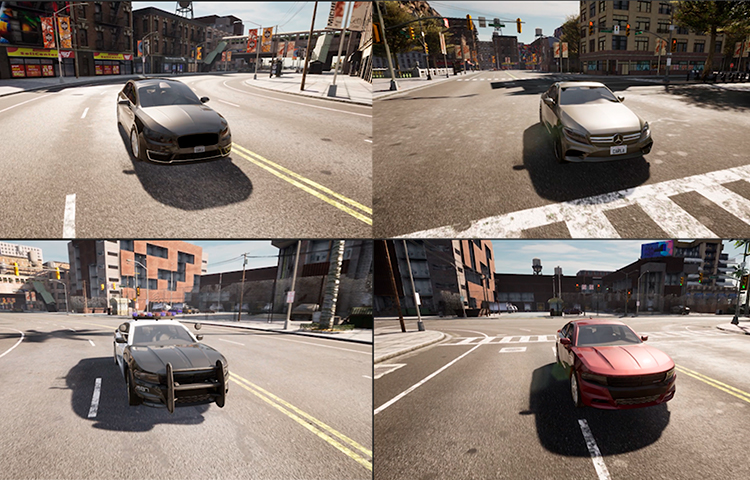
\includegraphics[height=8cm]{imagenes/cap3/carla.jpg}
	\end{center}
	\caption[Imagén de vehículos en CARLA]{Imagén de vehículos en CARLA}
	\label{fig:CARLA_vehicles}
\end{figure}

CARLA es una de las piezas clave de este \ac{TFG} es el escenario virtual en el que se desarrollan, prueban y evalúan todos los algoritmos y modelos diseñados para las problemáticas de conducción autónoma planteadas. \footnote{\url{https://carla.org/}}


\subsection{ROS 2}
\label{subsec:Ros 2}

ROS 2, la evolución de segunda generación de ROS, es un meta sistema operativo de código abierto diseñado específicamente para ser utilizado en robots. Proporciona servicios que se esperarían de un sistema operativo, incluyendo abstracción de hardware, control de dispositivos de bajo nivel e implementación de funcionalidades \cite{introducción_a_ros}. Una de las características fundamentales de ROS es su modelo de comunicación basado en el sistema publicador-suscriptor. En este sistema, los nodos (componentes individuales de software en un sistema ROS y ROS 2) pueden comunicarse entre sí de manera asíncrona. Un nodo que tiene información para compartir se convierte en un publicador y envía mensajes a un topic. Otros nodos que estén interesados en recibir esa información se suscriben a ese y recibirán los mensajes publicados en él. Esto permite una comunicación eficiente y flexible entre los diferentes nodos que conformen nuestro sistema.

\bigskip
\begin{figure} [H]
	\begin{center}
	
\includegraphics[height=3cm]{imagenes/cap3/ros2_logo.png}
	\end{center}
	\caption[logotipo de Ros 2]{Logotipo de Ros 2}
	\label{fig:Ros2_logos}
\end{figure}
\bigskip

En el desarrollo de este Trabajo de Fin de Grado, ROS 2 se utilizó para elaborar una sección específica del código y de los algoritmos de conducción autónoma. La decisión de integrar ROS 2 con el simulador CARLA tuvo un propósito muy claro: evaluar la viabilidad de unir las capacidades de este sistema, que es una referencia en el mundo de la robótica, con el entorno de simulación de conducción autónoma que CARLA ofrece. Esta integración se realizó con el objetivo de no solo generar algoritmos más robustos y eficaces sino también de explorar nuevas posibilidades y métodos para la creación de sistemas de conducción autónoma. Esta fusión entre ROS 2 y CARLA se convirtió en un elemento clave para entender y desarrollar más a fondo los complejos retos que plantea la conducción autónoma, permitiendo una interacción más fluida y adaptable entre los diferentes componentes del sistema. \footnote{\url{https://www.ros.org/}}

\bigskip 

\subsection{CARLA to ros bridge}
\label{subsec:CARLA to ros bridge}

\textit{CARLA to ros bridge} es una herramienta oficial desarrollada por el equipo de CARLA. Esta herramienta tiene el objetivo de ser,  un medio de comunicación bidireccional entre CARLA y un entorno de desarrollo ROS o ROS2. Por un lado el bridge de encarga de traducir la información de CARLA  a topics y mensajes de ROS de manera que el framework  pueda entenderlos sin mayor dificultad. Por otro lado el bridge se encarga también de traducir los mensajes publicados en los topics generados para CARLA en mensajes basados en la\ac{API} del simulador para que, de esta manera un nodo ROS 2 pueda comunicarse con CARLA como lo haría con cualquier robot. carla to ros bridge puede ser encontrado de su repositorio oficial de Github, en el aparte del código encontraremos instrucciones para su descarga y uso\footnote{\url{https://github.com/carla-simulator/ros-bridge}}
\begin{figure} [H]
	\begin{center}
	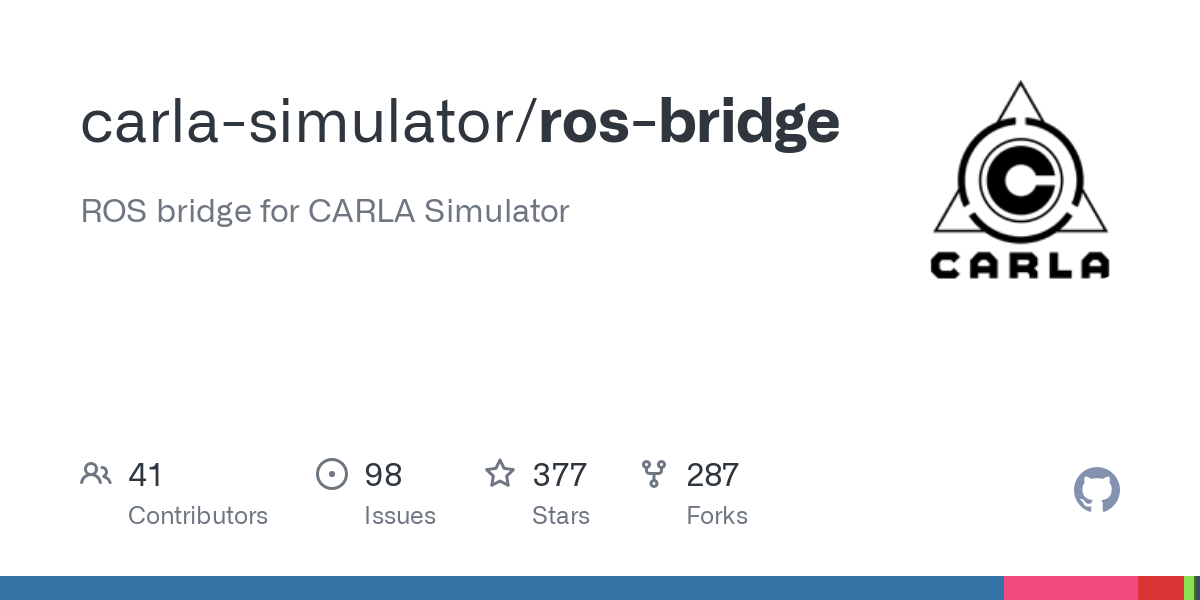
\includegraphics[height=6cm]{imagenes/cap3/carla_to_ros_bridge.png}
	\end{center}
	\caption[CARLA to ros bridge]{CARLA to ROS bridge}
	\label{fig:carla_to_ros_bridge}
\end{figure}
en este este \ac{TFG} carla to ros bridge ha tenido un papel fundamental  en la fase de investigación y experimentación sobre la viabilidad del desarrollo de algoritmos de conducción autónoma en ROS 2 para el simulador CARLA, permitiendo que CARLA y ROS 2 se comunicarán.


\subsection{Visual studio code}
\label{subsec:Visual studio code}

Visual studio code  \footnote{\url{https://code.visualstudio.com/}} es un editor de código gratis, ligero, profesional y fácil de usar disponible tanto para Linux, como para Windows, como para macOS. Probablemente representa la elección favorita de la gran mayoría de los programadores de hoy en día a la hora de eligir un editor de código. Tanto en ambientes de investigación como en entorno profesionales de producción de aplicaciones y programas Visual studio code es ampliamente conocido y utilizado.

\begin{figure} [H]
	\begin{center}
	
\includegraphics[height=4cm]{imagenes/cap3/vsc-logo.png}
	\end{center}
	\caption[carla to ros bridge]{Visual studio code logo}
	\label{fig:vcs logo}
\end{figure}

Visual studio code ha sido el editor elegido para la programación de todo el código de este \ac{TFG}. Los algoritmos, herramientas y aplicaciones que más tarde se explicarán han sido todas gestados en este famoso editor.

\subsection{PyTorch}
\label{subsec:PyTorch}

PyTorch \footnote{\url{https://pytorch.org/}} es una biblioteca de aprendizaje automático de código abierto desarrollada principalmente por el equipo de inteligencia artificial de Facebook. Es especialmente popular en la comunidad académica y de investigación por su flexibilidad y eficiencia. Compatible con sistemas operativos como Linux, Windows y macOS, PyTorch facilita tanto la investigación experimental como la implementación de modelos en producción. Su diseño intuitivo y las capacidades para realizar cálculos de tensores de manera eficiente lo convierten en una de las bibliotecas más utilizadas en aprendizaje profundo y visión por computadora. En entornos tanto académicos como profesionales, PyTorch es ampliamente reconocido y empleado para una variedad de aplicaciones que van desde el análisis de datos hasta el reconocimiento de imágenes y la robótica. Dentro del contexto de este \ac{TFG} Pytorch se utilizará para cargar y utilizar modelos de redes neuronales en algunas de las implementaciones

\subsection{OpenCV}
\label{subsec:OpenCV}

OpenCV \footnote{\url{https://opencv.org/}} es una biblioteca de visión por computadora de código abierto. Originalmente desarrollada por Intel, OpenCV es especialmente potente para tareas relacionadas con el procesamiento de imágenes, detección de objetos y funciones de realidad aumentada. Es una de las herramientas más utilizadas en el campo de la visión artificial debido a su accesibilidad, eficiencia y comunidad activa. Su amplio conjunto de funciones y utilidades lo hacen versátil y altamente funcional para una variedad de aplicaciones prácticas, desde sistemas de vigilancia y diagnóstico médico hasta vehículos autónomos. En este proyecto Opencv se utilizará como la biblioteca estándar para realizar todo el procesamiento de imágenes necesario para la implementación de los algoritmos y funcionalidades.


\subsection{Pygame}
\label{subsec:Pygame}

Pygame \footnote{\url{https://www.pygame.org/}} Según su página de Wikipedia oficial \cite{pygame}, Pygame es una biblioteca de Python que se utiliza para el desarrollo de videojuegos y aplicaciones multimedia interactivas. Es compatible con sistemas operativos como Linux, Windows y macOS, y su diseño sencillo y la amplia documentación disponible lo convierten en una de las bibliotecas más accesibles para empezar en el mundo del desarrollo de videojuegos. En entornos tanto educativos como de desarrollo indie, Pygame es ampliamente reconocido y utilizado para una variedad de proyectos, en el contexto de este \ac{TFG}, Pygame se utilizará para la implementación de las interfaces gráficas de todas las aplicaciones presentadas

\subsection{Servidor Landau de la Escuela de ingeniería superior de Fuenlabrada de la URJC}
\label{subsec:Servidor landau de la URJC}

Una de las principales limitaciones que los ingenieros nos encontramos a la hora de trabajar con \ac{IA}, es si duda, la necesidad de un hardware potente para el correcto funcionamiento de esta. La ejecución y entrenamiento de algoritmos de inteligencia artificial y aprendizaje automático suelen ser computacionalmente muy pesado lo cuál dificulta su ejecución de manera correcta y fluida sin el Hardware adecuado. Generalmente lo más importante en este aspecto es una \ac{GPU} potente. En el caso del \ac{TFG} que en esta memoria se presenta, existe el problema añadido de que como anteriormente se ha mencionado se utiliza el simulador foto-realista CARLA el cuál por otra parte también requiere un gran cantidad de memoria de \ac{GPU} para poder funcionar. Éstos dos factores hicieron que para realizar este \ac{TFG} fuera vital disponer de una \ac{GPU} muy potente capaz de correr CARLA y a la vez ser capaz de ejecutar algoritmos pesados de \ac{IA}.

\bigskip

Esta problemática hubiera sido probablemente uno de los problemas más grandes a los que este \ac{TFG} se hubiera tenido que afrontar, debido a que el hardware que se necesitaba era sumamente costoso y probablemente inasumible. Afortunadamente esto no fue así ya que la Escuela de ingeniería superior de la \ac{URJC} se ofreció a proporcionar el hardware necesario ofreciendo acceso a un servidor propio y privado de la Universidad el cuál permitía ejecutar código en racks de gráficas Nvidia alojadas en la misma universidad.

\bigskip

El servidor Landau de la Escuela de ingeniería superior de Fuenlabrada, perteneciente a la \ac{URJC} cuenta con 4 gráficas Nvidia A100 de 80 GB cada una. En la figura \ref{fig:graficas servidor landau} se puede ver la información de los recursos gráficos del servidor Landau obtenida del propio servidor mediante la ejecucióin del comando \textit{nvidia-smi}
\bigskip

\begin{figure} [H]
	\begin{center}
	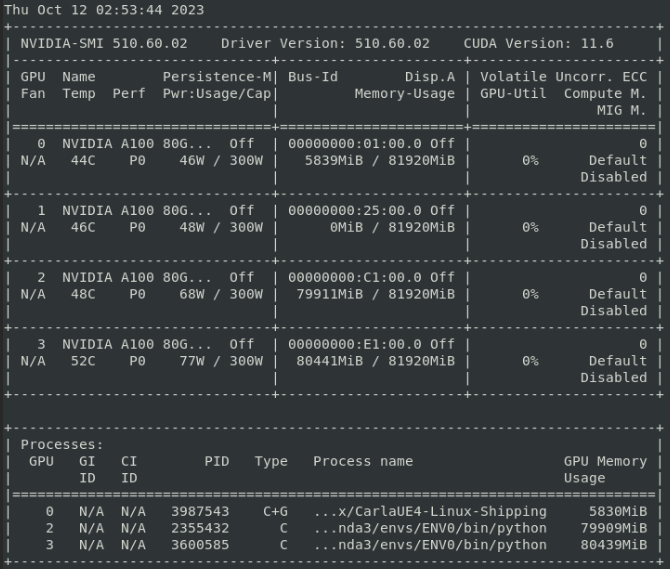
\includegraphics[height=9cm]{imagenes/cap3/graficas.png}
	\end{center}
	\caption[carla to ros bridge]{información de las GPU del servidor Landau}
	\label{fig:graficas servidor landau}
\end{figure}


\bigskip

De esta manera y después de que me fueran otorgados los permisos para acceder a este servidor, este se convirtió en un pilar casi imprescindible de este \ac{TFG} debido a que fue en esta plataforma donde se ejecutaron CARLA y todos los algoritmo y aplicaciones de conducción autónoma de una manera lo suficientemente fluida como para permitir un comportamiento reactivo.

\newpage
	









